\section{Analysis} \label{sec:Analysis}
\subsection{Calibrated Model}
We calibrated the model according to the previous section the calibration is reported in table \ref{tab:ModelCalib}.
\begin{table}[H]
\begin{adjustbox}{max width=\textwidth}
\begin{threeparttable}[b]
\caption{Parameters of the model}
\label{tab:ModelCalib}
\begin{tabular}{@{}lllcc@{}}
\toprule
 & Parameter                              & Notation         & Calibration & \citet{Campbell1999}\\ \midrule 
\multicolumn{5}{l}{\textit{Calibrated}}                                            \\
 & Mean consumption growth                & $g$              & $0.0134$  & $0.0189$\\
 & Standard deviation of $\Delta c_t$     & $\sigma$         & $0.0152$  & $0.0150$\\
 & Standard deviation of $\Delta d_t$     & $\sigma_w$       & $0.1256$  & $0.1120$\\
 & Log risk-free rate                     & $r^f$            & $0.0109$  & $0.0094$\\
 & Persistence parameter                  & $\phi$           & $0.9008$  & $0.8700$\\
 \multicolumn{5}{l}{\textit{Assumed}}                                              \\
 & Coefficient of Risk Aversion           & $\gamma$         & $2.0000$  & $2.0000$\\
 & Correlation dividends/consumption      & $\rho$           & $0.2000$  & $0.2000$\\
\multicolumn{5}{l}{\textit{Implied}}                                               \\
 & Subjective discount factor             & $\delta$         & $0.9156$  & $0.8900$\\
 & Steady-state surplus consumption ratio & $\Bar{S}$        & $0.0666$  & $0.0570$\\
 & Maximum surplus consumption ratio      & $S_{\text{max}}$ & $0.1096$  & $0.0940$\\ \bottomrule
\end{tabular}
\begin{tablenotes}
\footnotesize{\item [1] All relevant parameters are annualized
              \item [2] Calibrated parameters are estimated from data, assumed are chosen arbitrarily on the grounds of existing literature, while implied parameters are calculated from the calibrated/assumed parameters.}
\end{tablenotes}
\end{threeparttable}
\end{adjustbox}
\end{table}

Calibrating the model to the extended data suggests a higher persistence parameter, higher volatility of dividend growth and lower consumption growth, the implied surplus consumption parameters suggest a slightly higher overall surplus consumption in comparison to \cite{Campbell1999}. The difference is likely to stem from these 25 years of extra data. 

\subsection{Simulation}
From the calibrated model we simulate a chain of 100.000 monthly draws from the economy yielding 8.332 years of simulated time-series. We find in addition to the series that the procedure is extremely sensitive to the distribution of grid points. We use 10 equally distributed grid-points and an additional 6 just below $s_{max}$, consistent with the approach of \citet{Campbell1999}.


The simulated economy behaves well according to most measures, that is it is able to explain the equity-premium puzzle, which is known to cause problems in many models including the much used \textit{power-utility}-model. The \citet{Campbell1999} model solves this by introducing time-varying risk-aversion, this however causes the risk-aversion to diverge when the surplus-consumption ratio is close to 0, causing the model to generate risk-aversion amongst the agents in these periods to be implausibly high, as can be seen in figure \ref{RA} in appendix \ref{App:AFigu}, reporting local utility-curvature coefficients as high as 1230, which is in sharp contrast to empirical estimates of risk aversion in the US found to be between .75 and 2 found by \citet{SLFred2015} from the standard \textit{power-utility} model.

\begin{table}[H]
\centering
\caption{Simulated Moments}
\label{tab:simmom}
\begin{tabular}{@{}lllll@{}}
\toprule
Statistic                                               & \makecell{Consumption \\ Claim} & \makecell{Dividend \\ Claim} & \makecell{CC99-Calibration \\ Consumption Claim} & \makecell{CC99-Calibration\\ Dividend Claim} \\ \midrule
$\mathbb{E}\left(\Delta c \right)$                      &0.013504&0.011661&0.019024&0.017369\\
$\sigma\left(\Delta c \right)$                          &0.01243&0.10257&0.012268&0.09147\\
$\mathbb{E}r^f$                                         &0.010881&0.010881&0.0094&0.0094\\
$\mathbb{E}\left(r-f^f\right)/\sigma\left(r-r^f\right)$ &0.37625&0.23074& 0.43644                                       &         0.31764                            \\
$\mathbb{E}\left(R-R^f\right)/\sigma\left(R-R^f\right)$ & 0.4173   & 0.31102               &  0.4761                                      &      0.389                               \\
$\mathbb{E}\left(r-r^f\right)$                          &  0.048783                 &      0.045342          &         0.067377                               &        0.06472                             \\
$\sigma\left(r-r^f\right)$                              &     0.12965              &       0.19651           &   0.15438                                       &                  0.19651                     \\
$\mathbb{E}\left(p-c\right)$                          &     3.1123                &      3.157            &         2.8926                                 &             2.9161                          \\
$\sigma\left(p-c\right)$                              &       0.26201            &      0.28973          &   0.27676                                     & 0.29361                                    \\ \bottomrule
\end{tabular}
\end{table}



The risk-aversion shortcoming of this model is not the subject of our analysis, and hence are not further examined. The remaining series simulated from the model, and their moments of interest as reported in table \ref{tab:simmom} are well behaved, allowing us to examine the predictability of stock returns during times of simulated crisis.
\newline
\\
Based on NBER-recession data, we find that the US economy was in recession approximately 13.4\% of the period spanning January 1950 until December 2018.  In the model a recession implies that present consumption in low relative to habit, that is the value of $s_t$ is lower than the steady state value of surplus consumption $\Bar{s}$ - integrating over the density of $s_t$ yields that the simulated economy is in recession during 37\% of all observations, which indicates that $\Bar{s}$ might be misspecified. To correct $\Bar{s}$ we match the empirical business cycle behavior by numerical optimization of the $s_t$ density shown in figure \ref{fig:DistriSt}, such that the empirical and simulated economy is in recession roughly the same amount. The $\Bar{s}$-value matching the empirical business cycle, throughout denoted $\Bar{s}_{rec}$ \textit{or} ($\Bar{S}_{rec}$), is found to be $-3.18$ ($0.0415$). One additional recession threshold we denote as $\bar{s}_{2,rec}$ is chosen as to capture only the most extreme non-linearity of the relationship between surplus consumption and expected returns as presented in figure \ref{fig:SPCPD-a}.

\begin{table}[H] 
\centering
\caption{Business Cycle, Simulated and historic}
\label{tab:BC}
\begin{tabular}{@{\hspace{8mm}}ll@{\hspace{5mm}}ccc@{}}
\toprule
                       & \multicolumn{3}{c}{\textit{Simulated}} & \textit{Historic}  \\ \midrule
                                          & $\Bar{S}$       & $\Bar{S}_{REC}$ & $\Bar{S}_{2,REC}$&    \\ \cmidrule(l){2-4} 
        \textit{Value}                        & 0.067 & 0.042& 0.02 &              \\
Recession,                                      \% &36.92 & 13.41 &2.83  & 13.41\\ \bottomrule
\end{tabular}
\end{table}




\begin{figure}[H]
    \centering
    \caption{Distribution of simulated $s_t$ chain}
    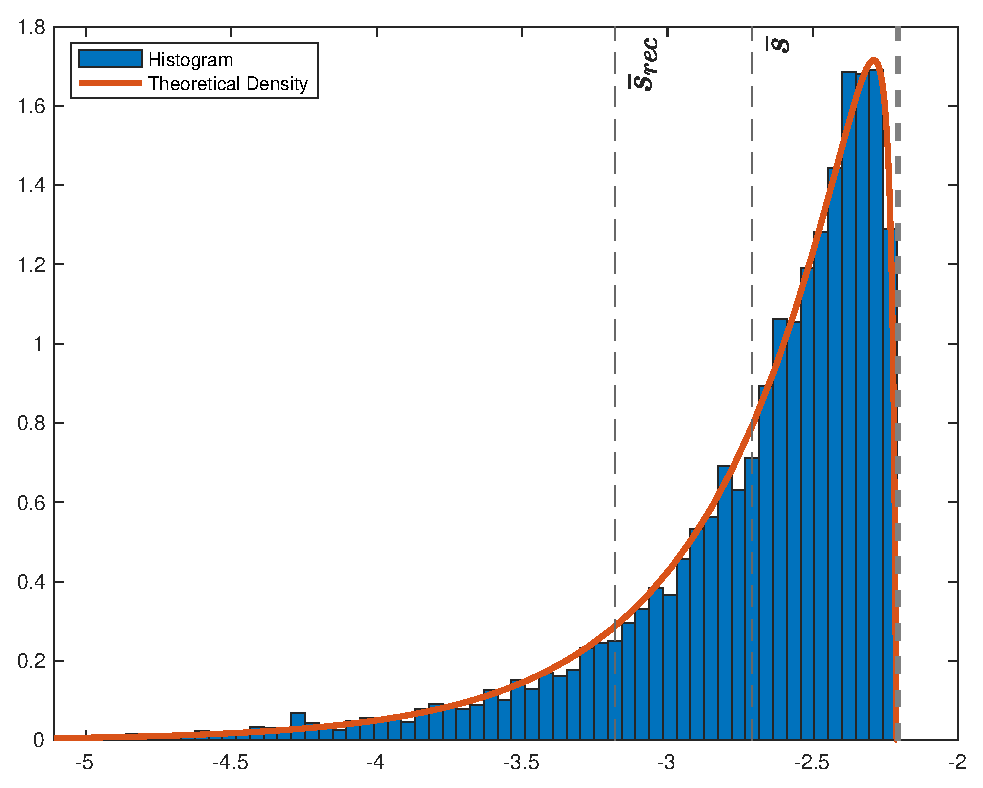
\includegraphics[width=\textwidth]{Figures/DistributionS_t.eps}
    \fnote{Histogram of the simulated $s_t$ or $\log(S_t)$, along with the continuous time density as derived by \citet{appendix}.}
    \label{fig:DistriSt}
\end{figure}
From the constructed surplus consumption threshold $\Bar{s}_{rec}$ for recession, we construct an indicator dummy for recessions. Such that $I_{rec} = 1$ \textit{if}. $\Bar{s}_{rec} > s_t$ and $I_{rec}=0$ otherwise.

Having simulated an economy based upon habit formation, and justified our choice of recession periods of the simulated series, we are able to test the proposed hypothesis:
\begin{enumerate}
    \item Is the model of \citet{Campbell1999} able to generate stock returns with the following two properties
    \begin{enumerate}
        \item Returns are predictable by the price/consumption- or the price/dividend-ratio under recessionary periods?
        \item Returns are unpredictable by the price/consumption- or the price/dividend-ratio under expansionary periods?
    \end{enumerate}
\end{enumerate}
Examining the expected returns as a function of the surplus consumption ratio, as in figure \ref{fig:SPCPD-a}. The model reveals a somewhat linear relationship for high values of the surplus consumption, the relationship however is much more steep and nonlinear when $S_t$ approaches ${S}_{REC}$, the goal is then to exploit this fact when predicting returns.


\begin{comment}
\begin{figure}[H]
    \centering
    \caption{Expected returns as a function of $S_t$}
    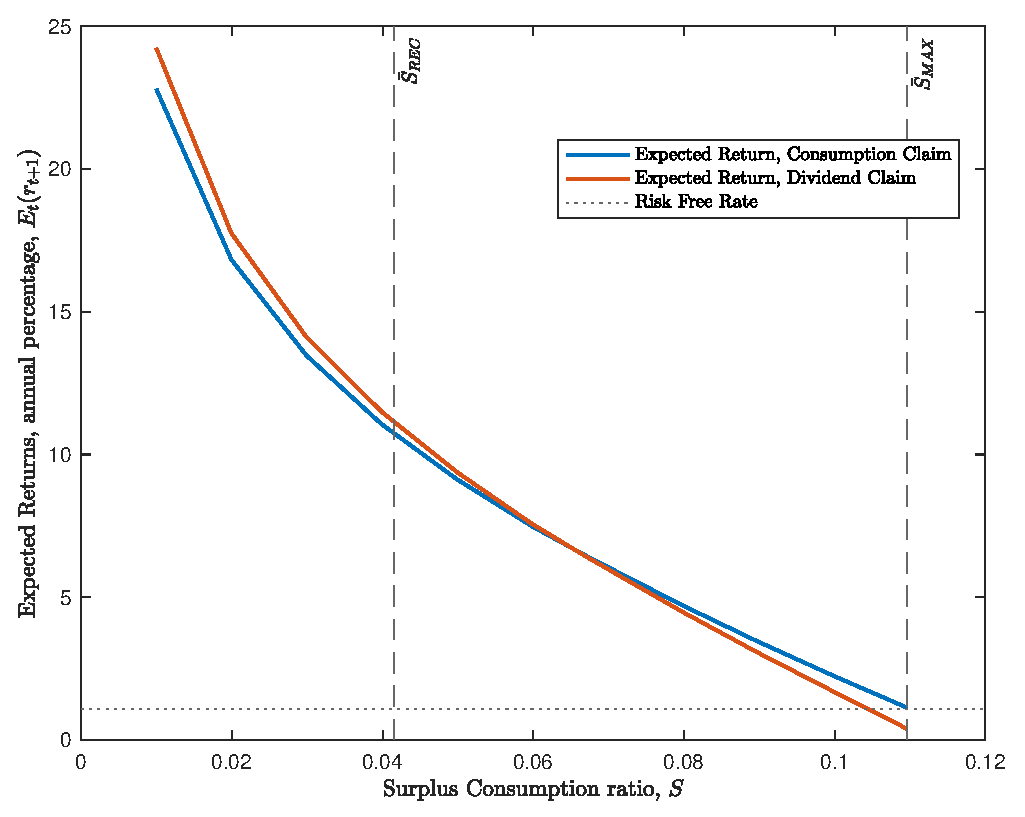
\includegraphics{Figures/ErPCPD.eps}
    \label{fig:ErPCPD}
\end{figure}
\end{comment}


\begin{figure}[H]
\centering
\caption{Functionals of surplus consumption ratio}
    \label{fig:SPCPD}
\subfigure[Expected returns as a function of $S_t$]{\label{fig:SPCPD-a}
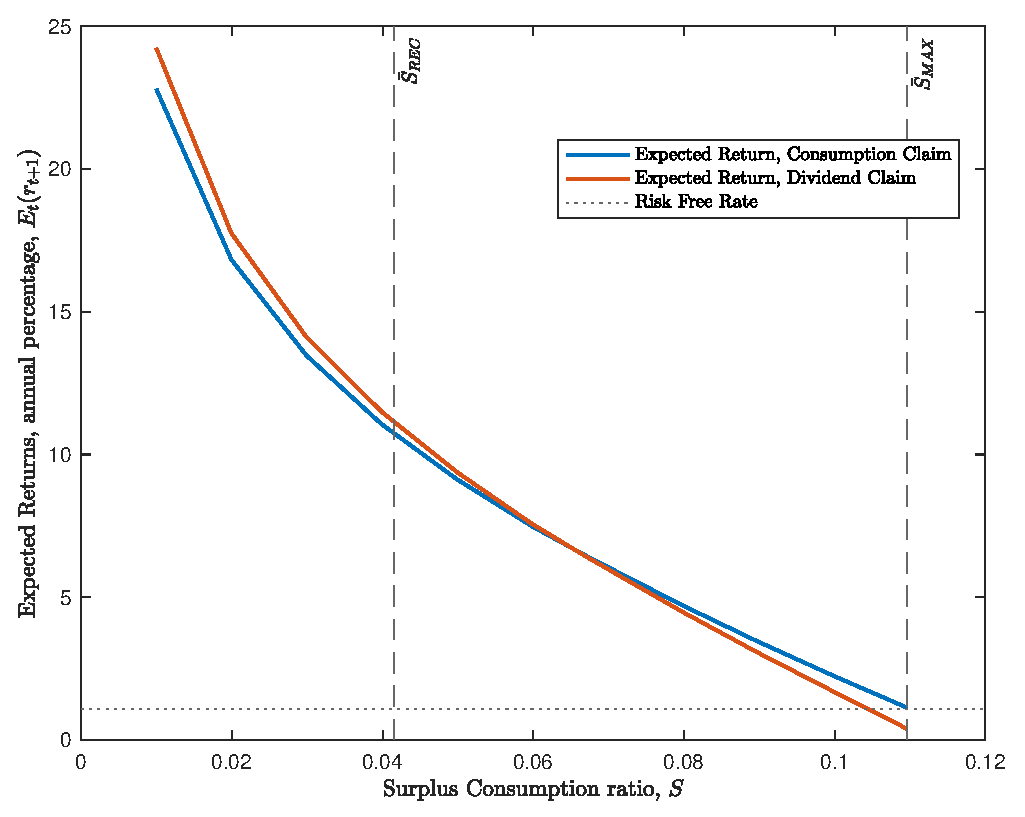
\includegraphics[width=0.45\textwidth]{Figures/ErPCPD.eps}} ~
\subfigure[$P/C$, $P/D$ as a function of $S_t$]{
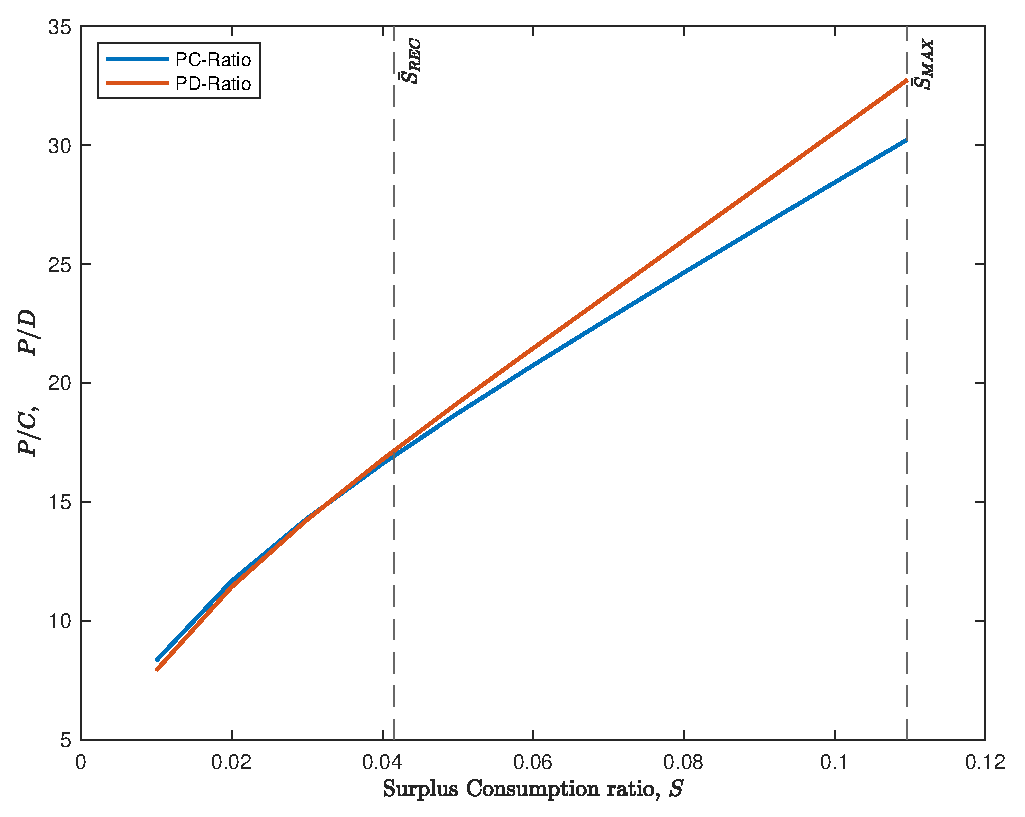
\includegraphics[width=0.45\textwidth]{Figures/PC_PD_Ratio.eps}}
\end{figure}

From the functionals of surplus consumption ratio reported in figure \ref{fig:SPCPD}, some basic predictions can be made. We see that when surplus consumption is low, that is in recessionary times, expected returns increases, the intuition is that when times are bad, as consumption falls relative to habit levels, the risk aversion increases, people wants a higher level of compensation per unit of risk - the risk premium rises - note that this must hold true for all levels of $S$ as the risk-free rate is fixed in the model. \\
Furthermore the figure implies that the regression coefficient of $P/C$ or equivalent $P/D$ should be negative. Lower P/C or P/D implies higher values of $\mathbb{E}\left[r_t-r^f\right]$, both driven by the single state.  


\subsection{Results}

First we estimate the following regressions:

\begin{align}
     r_{t+1} - r^{f} &= \alpha + \beta_{REC} \left( p_t - c_t \right) * I_{t,REC} + \beta_{EXP} \left( p_t - c_t \right) * \left(1 - I_{t,REC}\right)  + \varepsilon_{t+1} \label{23}\\
      r_{t+1} - r^{f} &= \alpha + \beta_{REC} \left( p_t - d_t \right) * I_{t,REC} + \beta_{EXP} \left( p_t - d_t \right) * \left(1 - I_{t,REC}\right)  + \varepsilon_{t+1} \label{24}\\
      r_{t+1} - r^{f} &= \left(\alpha_{REC} + \beta_{REC} \left(p_t - c_t\right)\right)*I_{REC}\dots \nonumber\\
      & + \left(1-I_{REC}\right) \left( \alpha_{EXP}\dots + \beta_{EXP}\left(p_t - c_t \right) \right) + \varepsilon_{t+1} \label{25}\\
r_{t+1} - r^{f} &= \left(\alpha_{REC} + \beta_{REC} \left(p_t - d_t\right)\right)*I_{REC}\dots \nonumber\\
& + \left(1-I_{REC}\right) \left( \alpha_{EXP} + \beta_{EXP}\left(p_t - d_t \right) \right) + \varepsilon_{t+1} \label{26}      
\end{align}



That is we use the recession indicator to infer the influence of the predictors in respectively recessions and expansions.\\

The regressions \eqref{25} and \eqref{26} are estimated over two steps; once for expansions and once for recessions. By these 2 pairs of regressions we estimate excess returns with a both with a constant intercept during all business cycle phases and in addition where we allow the intercept to change over business-cycles such that the slope is not the only thing driving predictability differences over recessions and expansions.


As a benchmark we estimate two additional regressions given by given:
\begin{align*}
     r_{t+1} - r^{f} &= \alpha + \beta \left( p_t - c_t \right)  + \varepsilon_{t+1}\\
      r_{t+1} - r^{f} &= \alpha + \beta \left( p_t - d_t \right) + \varepsilon_{t+1}
\end{align*}

Figure \ref{tab:regress1} reports results of the four regressions. The desired property of separability of predictability during phases of the business cycles gains some support from this result. We see a significant increase in $R^2$, we find strong statistical evidence supporting rejection of the null-hypothesis for all estimates in all four regressions, this is however to be expected as a sample size of between 12.000 and 100.000 observations is quite large, it is well established that as the sample size increases the asymptotic variance of the OLS-estimate decreases and thus significance is inevitable as the sample size becomes quite large.


\begin{table}[H]
\centering
\caption{Regressions, $\Bar{S}_{REC} = 0.041542$}  
\label{tab:regress1}
\begin{threeparttable}
\begin{tabular}{@{}lccccccc@{}}
\toprule
& \multicolumn{6}{c}{\textit{Dependent variable: $r^{e}_{t+1}$}} \\ 
\midrule
& \multicolumn{3}{c}{Dividend Claim} && \multicolumn{3}{c}{Consumption Claim} \\
\cmidrule(lr){2-4} \cmidrule(lr){6-8}
Constant & 0.09133  & 0.2174  & 0.1466  & & 0.08802 & 0.1828 & 0.1451 \\
         & (0.0066) & (0.015) & (0.0067)& &(0.0055) & (0.013)& (0.0049)\\
\addlinespace
$\beta_{REC}$ &-0.01589  & -0.04198 &&& -0.01529 & -0.03507 & \\
              & (0.0013) & (0.003)  &&& (0.0011) & (-0.0025) & \\
\addlinespace 
$\beta_{EXP}$ & -0.01547 & & -0.02497&& -0.01496 && -0.02488\\
              & (0.0011) & & (0.0012)&& (0.00095) && (0.00085)\\
\addlinespace
\midrule
$R^2$,~\%         & 0.48 & 1.9 & 0.58 & & 0.84 & 2.2 & 1.2 \\
\bottomrule
\end{tabular}
\begin{tablenotes}\footnotesize{
\item[1] Brackets below estimates contains \citet{NW87} corrected standard errors. 
\item[2] Expansionary observations: 85950, recessionary observations: 12220, full-sample (\textit{including overlaps}) 99999
\item[3] All variables in logs}
\end{tablenotes}
\end{threeparttable}
\end{table}

We then run the empirical counterpart to this regression using the same data as we used in the calibration of the model. We use the \textit{30-day} T-bill as the risk-free rate and the NBER \textit{US} recession indicator, note that as to remain true to realistic empirical studies the risk-free rate is not considered to be constant for the purpose of this regression. 

\begin{table}[H]
 \centering
   \caption{Empirical dividend-price regressions}           
   \label{tab:regressEmp}
 \begin{threeparttable}
 \begin{tabular}{@{}ccccccc@{}}
 \toprule
   \multicolumn{3}{c}{Recession} && \multicolumn{3}{c}{Expansion} \\ 
 \addlinespace
 Constant  & $\beta$  &  $R^2,\%$     && Constant & $\beta$   &  $R^2$,\%      \\
 \cmidrule(lr){1-3} \cmidrule(lr){5-7}
 0.191  & $-$0.032 & 4.42             && 0.015    & $-$0.00001  & 0.47           \\ 
 \addlinespace
 (0.0907)  & (0.0159) &               && (0.0043) & (0.0000)  &                \\
 \bottomrule
 \end{tabular}
 \begin{tablenotes}\footnotesize{
 \item[1] Brackets below estimates contains \citet{NW87} corrected standard errors \textit{1 lag}. 
 \item[2] Regressions on monthly data spanning Jan. 1950 - Dec. 2018.
 \item[3] All variables in logs
 }
 \end{tablenotes}
 \end{threeparttable}
 \end{table}

The slope of the price-dividend ratio during recessions is of the same magnitude as the one estimated from the simulated economy (.035 vs. -0.032) same goes for the constant in receessions. This result follows from column 2 of the consumption claim part of table \ref{tab:regress1}. The expansionary slope coefficient deviates quite a lot, we see how $\beta_{EXP}\approx 0$, implying that during expansions price dividend ratio has zero impact on excess returns. In the model however the correlation between excess returns and the price-dividend ratio is inevitable. We see this clearly from figure \ref{fig:SPCPD}, where even out of recessions the inverse almost linear relationship is quite strong.


To examine whether this results holds \textit{out-of-sample}, we conduct a rolling-window forecast over the simulated observations. As the underlying $s_t$-chain leads to realistic economic business cycles and thus non-continous chains of recessions, we stack all recession periods to one sample, this is justified in the model as the state variable $s_t$ behaves consistently and the behavior of the remaining series behaves according to $s_t$, that is we have no structural changes over \textit{t} in the model. \\
We use the squared forecast errors to estimate the $R^2_{OoS}$ as \citet{CT2005}, the computed $R^2_{OoS}$ is reported in table \ref{tab:R2OS}. 

\begin{table}[H]
\centering
\caption{Out-of-sample $R^2$}
\label{tab:R2OS}
\begin{threeparttable}
\begin{tabular}{@{}lccccc@{}}
\toprule
                         & \multicolumn{2}{c}{Dividend Claim} && \multicolumn{2}{c}{Consumption Claim} \\ 
                         \addlinespace
& Expansions       & Recessions      && Expansions        & Recessions        \\
\cmidrule(lr){2-3} \cmidrule(lr){5-6}
$R^2_{OoS}$, \textit{\%} & -1.22            & 1.04            && -0.88             & 1.07              \\ \bottomrule
\end{tabular}
\begin{tablenotes}\footnotesize{
\item[1] Based upon 1-\textit{period-ahead} rolling-window forecast with a window size of 120 months.
\item[2] Expansionary observations: 85218, recessionary observations: 11488}
\end{tablenotes}
\end{threeparttable}
\end{table}

The interpretation is that the simple forecast of excess returns using the price-consumption ratio or equivalently price-dividend ratio compared to the no-predictability forecast, the mean-model forecast of excess returns, the simple regression performs better only in recessionary periods, while the mean-model is superior in times of economic prosperity. For our hypothesis this result is good news, in times of expansion price-dividend ratio does not predict excess stock returns out-of-sample, while the opposite remains true in recessions.\\


However from figure \ref{fig:SPCPD-a} we see that the most extreme effect of $S_t$ on expected returns kicks in at an estimated $0.02$, based on this fact we run additional regressions with the same specification as above, but with a respecifed $\Bar{S}_{REC}=0.02$ and denote this $\bar{S}_{2,REC}$, the output of which is reported in table \ref{tabregress2}. This specification of $\Bar{S}_{REC}$ implies that the simulated economy is in recession approximately 2.8\% of the time. Corresponding to barely 3.000 observations in this case. \\
\newline


This specification indicates that recessions are defined now as only the most severe times of the simulated economy. The surplus consumption is extremely low, the threshold value of 0.02 indicates relative levels of risk aversion in this periods of at least 100, which is huge, leading to expected  returns of above 17\%. This gives us an idea of the state of the economy. The intuitive predictions based upon the model framework is that we should obtain similar results to those of table \ref{tab:regress1}, however with the effect of price-dividend ratio on excess returns in recessions being much larger and even more predictability in recessions.

\begin{table}[H]
\centering   
  \caption{Benchmark regressions}           
  \label{tab:regress1}     
  \begin{threeparttable}
\begin{tabular}{@{\hspace{5pt}}l@{\hspace{15pt}}c@{\hspace{5pt}}c} 
\toprule 
 & \multicolumn{2}{c}{\textit{Dependent variable:}} \\ 
 & \multicolumn{2}{c}{$\left(r_{t+1}-r^f\right)$} \\ 
 \cmidrule(rr){2-3}
 & (1) & (2)\\ 
\midrule  
\\[-2.1ex] $ p_t - c_t $ &-0.1516&\\ 
  & (0.0071) &  \\ 
 \addlinespace 
  $p_t - d_t $ & &   -0.137 \\ 
               & &  (0.0064) \\ 
 \addlinespace 
 Constant &0.5206 &0.4814\\ 
          &(0.023) &(0.021) \\ 
 \addlinespace 
\midrule  
Observations & 8331 & 8331\\
R$^{2}$ &0.094 & 0.094 \\ 
Residual Std. Error &0.015 & 0.015 \\ 
\bottomrule 
\end{tabular} 
\begin{tablenotes}
\footnotesize{
\item[1] Brackets below estimates contains Newey-West corrected standard errors. 
\item[2] Regressions on 8331 years of simulated data.
\item[3] EXP (REC) denotes expansion (recession)
}
\end{tablenotes}
\end{threeparttable}
\end{table} 


\begin{table}[H]
\centering
\caption{Regressions, $\Bar{S}_{REC} = 0.02$}  
\label{tab:tabregress2}
\begin{threeparttable}
\begin{tabular}{@{}lccccccc@{}}
\toprule
& \multicolumn{6}{c}{\textit{Dependent variable: $r^{e}_{t+1}$}} \\ 
\midrule
& \multicolumn{3}{c}{Dividend Claim} && \multicolumn{3}{c}{Consumption Claim} \\
\cmidrule(lr){2-4} \cmidrule(lr){6-8}
Constant & 0.07881  & 0.3536  & 0.09586 && 0.07811 & 0.3112 & 0.09567 \\
         & (0.0066) & (0.039) & (0.005) &&(0.005) & (0.033)& (0.0039)\\
\addlinespace
$\beta_{REC}$ &-0.01316  & -0.07347 &&& -0.0132    & -0.06462 & \\
              & (0.0011) & (0.0083)  &&& (0.00088) & (-0.007) & \\
\addlinespace 
$\beta_{EXP}$ & -0.0133 & & -0.01626   && -0.01323  && -0.01631\\
              & (0.00088) & & (0.00087)&& (0.00071) && (0.00069)\\
\addlinespace
$R^2$,~\%         & 0.47 & 3.3 & 0.45 & & 0.86 & 3.8 & 0.86 \\
\bottomrule
\end{tabular}
\begin{tablenotes}\footnotesize{
\item[1] Brackets below estimates contains \citet{NW87} corrected standard errors. 
\item[2] Expansionary observations: 96435, recessionary observations: 2972, full-sample (\textit{including overlaps}) 99999}
\end{tablenotes}
\end{threeparttable}
\end{table}



\begin{table}[H]
    \centering
    \caption{Long Run Regressions}
   \begin{tabular}{l@{\hspace{8mm}}cccc}
   \toprule
\textit{Horizon, Years}& $\beta_{pc}$ & $R^2_{pc}$ & $\beta_{pd}$ & $R^2_{pd}$ \\ 
\midrule
1 & -0.135 & 0.0736 & -0.122 & 0.0735 \\ 
2 & -0.273 & 0.1574 & -0.247 & 0.1572 \\ 
3 & -0.398 & 0.2324 & -0.360 & 0.2321 \\ 
5 & -0.617 & 0.3580 & -0.558 & 0.3576 \\ 
7 & -0.790 & 0.4525 & -0.714 & 0.4521 \\ 
10 & -0.979 & 0.5492 & -0.885 & 0.5488 \\ 
\bottomrule 
\end{tabular}
    \label{tab:LHREGRESSION}
\end{table}

\begin{comment}
\midrule
1 & -0.13493 & 0.073631 & -0.12195 & 0.073542 \\ 
2 & -0.27306 & 0.15742 & -0.2468 & 0.15724 \\ 
3 & -0.39824 & 0.23238 & -0.35995 & 0.23213 \\ 
5 & -0.61689 & 0.35796 & -0.55757 & 0.35757 \\ 
7 & -0.78972 & 0.45245 & -0.71386 & 0.45206 \\ 
10 & -0.9792 & 0.54915 & -0.88524 & 0.5488 \\ 
\bottomrule 
\end{comment}
\begin{comment}
Instead we run a regime-switching linear regression with observable states, remember that from the simulation we obtained the surplus consumption ratio as an observable. In real data one would have to rely on latent state regressions such as a \textit{hidden Markov model}, to determine the latent state as a function of $s_t$.\\
However we have the simulated series and are able to run the regression straightforward. We run four regressions again with excess stock return as the regressand:

\begin{align*}
    \left(r_{t+1} - r^{f}\right) I_{t+1,REC} &=  \alpha + \beta \left( p_t - c_t \right) I_{REC,t} + \varepsilon_{t+1}\\
    \left(r_{t+1} - r^{f}\right)I_{t+1,REC} &=  \alpha + \beta \left( p_t - d_t \right) I_{REC,t} + \varepsilon_{t+1}\\
    \left(r_{t+1} - r^{f}\right)I_{t+1,EXP} &=  \alpha + \beta \left( p_t - c_t \right) \left( 1- I_{REC,t}\right)  + \varepsilon_{t+1}\\
    \left(r_{t+1} - r^{f}\right)I_{t+1,EXP} &=  \alpha + \beta \left( p_t - d_t \right) \left( 1- _{REC,t}\right) x+ \varepsilon_{t+1}
\end{align*}


The results of the four regressions are reported in table \ref{tab:RSregress}, the results are quite interesting. Examining the results reveals that with a regime switching approach as opposed to the previous single state regression, we are able to split the effects of business cycles on the predictability of stock returns. Notice how the coefficients indicating the effects of respectively P/C and P/D ratios on excess returns have switched signs in recession periods, while the constant effect is negative during recessions, indicating the base effect of being in a recession on excess returns is negative. However while not intuitively inappropriate in this context it have to be noted that expected returns are restricted to be positive in this model, therefore mandating that the size of the log P/C and log P/D-ratios must be large enough to offset the negative constant. This restriction is not particular restrictive as the log price consumption-ratio and equivalent log price dividend ratio is seldom below 2, see the simulated chains of log P/C and log P/D in figure \ref{fig:PCPD} in appendix.\\

Another result worth noting is one that provides evidence in favor of both of our hypothesis, that is the estimated coefficient of determination is much higher in the recession periods reaching 7\% when predicting excess returns using the price-consumption-ratio, than it is in expansionary periods reaching just barely .2\%, using the price-dividend-ratio as the predictor yields a smaller $R^2$ this is to be expected, as the price-dividend is by construction a noisier mapping of the price-consumption-ratio dynamics, containing not only the shock to consumption growth $\sigma$ but also the shock to dividend growth $\sigma_w$.\\

Now in real data it is not plausible to condition the regressand on a future variable like we do with the recession indicator. The reason why it is still not completely unreasonable is the high persistence of $s_t$, remember that $s_t$ is driven by the highly persistent growth rate of consumption, estimating the persistence in our simulation yields an autocorrelation coefficient of $0.9972$. From our monthly simulated series of $s_t$ the mean length of recessionary periods is around 1.2 years based upon the $\bar{s}_{rec}$, while the empirical mean length of recessions is around 0.93 years based on monthly NBER-recession data. Implying that real business cycles is not quite as persistent as in the model, or rather that the surplus consumption ratio might not be the sole determinant of recessions in reality, however a difference in average recession length of 3 months does not seem to bad.

In real data it would be more reasonable to estimate a transition probability matrix to forecast the underlying business cycle chain, and condition on the recession forecast. Recession forecasts, however, are notoriously unreliable, contaminating the estimates with very high levels of uncertainty.

\begin{table}[H]
\centering   
  \caption{Regime Switching Regression}           
  \label{tab:RSregress}     
  \begin{threeparttable}
\begin{tabular}{@{\hspace{5pt}}l@{\hspace{5pt}}cccc} 
\toprule 
 & \multicolumn{4}{c}{\textit{Dependent variable:}} \\ 
 & \multicolumn{2}{c}{$\left(r_{t+1}-r^f\right)_{REC}$} & \multicolumn{2}{c}{$\left(r_{t+1}-r^f\right)_{EXP}$} \\ 
 \cmidrule(rr){2-5}
 & (1)   &   (2) & (3) & (4) \\ 
\midrule  
\\[-2.1ex] $ p_t - c_t $ & 0.001174&  &-0.0003139   & \\ 
  & (9.4e-05) & &(3.6e-05) & \\ 
 \addlinespace 
 $p_t - d_t$ &  & 0.001168 & &-0.000323 \\
 & & (9.4e-05) & &(3.523e-05) \\
 \addlinespace 
 Constant &-0.0005367 &-0.0005311 &0.00537 &0.005429 \\ 
  &(2.3e-05) &(2.3e-05) &(0.00018) &(0.00018) \\ 
 \addlinespace 
\midrule  
Observations & 99999 & 99999 & 99999 &99999\\ 
R$^{2}$ &0.009 & 0.0089 & 0.00036 &0.00039\\ 
Residual Std. Error &0.00045 & 0.00045 &0.001 & 0.001  \\ 
\bottomrule 
\end{tabular} 
\begin{tablenotes}
\footnotesize{
\item[1] Brackets below estimates contains \citet{NW87} corrected standard errors. 
\item[2] Regressions on 99999 months of simulated data.
\item[3] EXP (REC) denotes expansion (recession)
}
\end{tablenotes}
\end{threeparttable}
\end{table} 


\begin{table}[H]
\centering
\caption{Simulated Moments}
\label{tab:MMoomme}
\begin{tabular}{@{}llllllllll@{}}
\toprule 
 & $\mathbb{E}\Delta d$ & $\sigma_{\Delta d}$ & $\mathbb{E}r^f$ & $\mathbb{E}r^m/\sigma _{r^m}$ & $\mathbb{E}R^m/\sigma _{R^m}$ & $\mathbb{E}r^m$ & $\sigma_{r^m}$ & $\mathbb{E}d-p$ & $\sigma_{d-p}$  \\ 
\midrule 
\multicolumn{10}{l}{$P/D$}\\
 &0.011661&0.10257& 0.010881 & 0.19839 & 0.27412 & 0.034063 & 0.1717 & 3.4246 & 0.21183 \\ 
\multicolumn{10}{l}{$P/C$}\\
 &0.013504&0.01243& 0.010881 & 0.38534 & 0.42038 & 0.037242 & 0.096645 & 3.3797 & 0.1864 \\ 
\bottomrule 
\end{tabular}

\end{table}



\begin{table}[H]
\centering
\caption{Data Properties}
\label{tab:Data_props}
\begin{tabular}{@{}l@{\hspace{1.5cm}}l@{\hspace{1.5cm}}l@{}}
\toprule
 & \textit{Simulated} & \textit{Historic} \\ \midrule
$\mathbb{E}\left[r_t- r^f_t\right]$& $0.0373$           & $0.0927$          \\
$\sigma\left(r_t - r^f_t  \right)$ & $0.0962$           & $0.1670$          \\
$\mathbb{E}\left[r_t- r^f_t\right] / \sigma\left(r_t - r^f_t,\right)$ & $0.3877$ & $0.5548$  \\ \bottomrule
\end{tabular}
\end{table}
\end{comment}

\subsubsection{Robustness}


\subsection{Economic Interpretation}


The economic interpretation follows from the model intuition. We see how in times of recession the risk-aversion increases exponentially, this implies that as we set the threshold for recessions lower in the model, the predictability of stock returns during recessions increases. That is the marginal contribution of predictability of the dividend claim in recessions decreases as surplus consumption relative to habit level increases. Using the model implied threshold of ${\BAR{S}}$ leads to little to no difference in predictability over business cycles. The empirically implied threshold leads to statistically significant differences, while lowering the threshold even further magnifies the results. \\


People exposed to significant losses, thus fearing further losses, increases the premium they demand for participating in a risky gamble; their risk-premium, this result is well established, but notoriously difficult for models to match. Augmenting the simple \textit{power-utility} model with external habit formation incorporates this feature, but with the cost of a bad-behaved risk-aversion series as can be seen in figure \ref{RA} in appendix \ref{App:AFigu}.


